\documentclass[tikz]{standalone}

\usetikzlibrary{angles, quotes}
\usetikzlibrary {arrows.meta}
\begin{document}
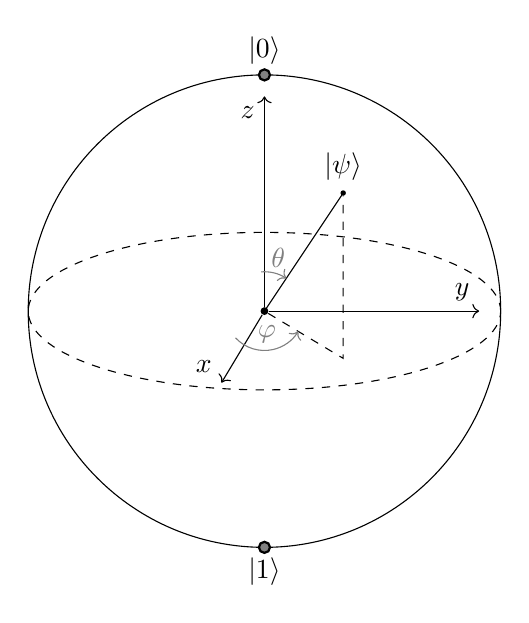
\begin{tikzpicture}

  % Define radius
  \def\r{3}

  % Bloch vector
  \draw (0,0) node[circle, fill, inner sep=1] (orig) {} -- (\r/3,\r/2)
    node[circle, fill, inner sep=0.7, label=above:$|\psi\rangle$] (a) {};
  \draw[dashed] (orig) -- (\r/3, -\r/5) node (psi) {} -- (a);

  % Sphere
  \draw (orig) circle (\r);
  \draw[dashed] (orig) ellipse (\r{} and \r/3);

  % Axes
  \draw[->] (orig) -- ++(-\r/5/1.1, -\r/3/1.1) node[above left] (x) {$x$};
  \draw[->] (orig) -- ++(\r/1.1, 0) node[above left] (y) {$y$};
  \draw[->] (orig) -- ++(0, \r/1.1) node[below left] (z) {$z$};

  % Angles
  \pic [draw=gray, text=gray, ->, "$\varphi$"] {angle = x--orig--psi};
  \pic [draw=gray, text=gray, <-, "$\theta$", angle eccentricity=1.4] {angle = a--orig--z};

  \filldraw[color=black, fill=gray, thick](0,\r) circle (2pt) node [above, black] {$|0\rangle$};
  
  \filldraw[color=black, fill=gray, thick](0, -\r) circle (2pt) node [below, black] {$|1\rangle$};
  
\end{tikzpicture}
\end{document}